%%-----------------------------------------------------------------------%%
%% This template was created by Celeste Damiani
%% for the training session "LaTeX for writing your thesis"
%% at Queen Mary University of London, April 2021.
%%-----------------------------------------------------------------------%%
%% This is your master document. Use as a dashboard to your project

%% Preamble
%%----------------------------------------------------------------------------------
\RequirePackage[l2tabu, orthodox]{nag} % nag will show warnings if you're using obsolete or deprecated commands. Optional.

\documentclass[12pt, a4paper, oneside]{book}


% languages, fonts and geometry
%------------------------------------------------------------------------------------
\usepackage[utf8]{inputenc}
\usepackage[italian, main = english]{babel} 			% manages typographical rules and hyphenation for the option languages
\usepackage[T1]{fontenc}							% manages font encoding (accents, copy and paste, ...)

\usepackage{titlesec, color}
\definecolor{gray75}{gray}{0.75}
\newcommand{\hsp}{\hspace{6pt}}
\titlespacing{\chapter}{0pt}{-50pt}{12pt}% left space, top space, bottom space
\titleformat{\chapter}[hang]{\Large\bfseries}{Chapter \thechapter:\hsp}{0pt}{\Large\bfseries}

\titleformat{\section}[hang]{\large\bfseries}{ \thesection\hsp}{0pt}{\large\bfseries}

\titleformat{\subsection}[hang]{\bfseries}{ \thesubsection\hsp}{0pt}{\bfseries}

% support for chinese
\usepackage{xeCJK}


% Load the parskip package without options
\usepackage{parskip}

%%-----------------------------------------------------------------------%%
%% from QM Guidance Notes on the Submission:
%% margins at the binding edge must be not less than 40 mm (1.5 inches)
%% and other margins not less than 20 mm (.75 inches). Double or one-and-a-half
%% spacing should be used, except for indented quotations or footnotes where single
%% spacing may be used. 
%%-----------------------------------------------------------------------%%


\usepackage[ 
		layoutoffset=0pt,						% No offset on the margins of the page
		bottom=2.5cm, 
		top=2.5cm,	
		left=2.5cm, 
		right=2.5cm,			
		bindingoffset=0pt,						% We already set a bigger binding edge margin
		headheight=26pt				% top space dedicated to the header
		]{geometry}	
					
\usepackage{microtype, fancyhdr}	 % typesetting adjustments
\usepackage{setspace}					 %allows local control over line spacing
\usepackage{pdflscape} 					 % makes landscape pages display as landscape when opening the pdf


%maths
%------------------------------------------------------------------------------------
\usepackage{amsfonts,amsmath,amsthm,amssymb, mathrsfs, amscd}	 %maths formatting
\numberwithin{equation}{chapter}	
%\numberwithin{table}{chapter} 
%\numberwithin{figure}{chapter}
\usepackage{faktor}
\allowdisplaybreaks

%tools
%------------------------------------------------------------------------------------
\usepackage{url, enumitem} 			% for linkable urls and nice lists
% \usepackage[noadjust]{cite}				% biblio management
\usepackage{epigraph}						% self explanatory
\usepackage[nottoc]{tocbibind}			% to make the bibliography appear in the ToC
\usepackage{blindtext}						% this is just to generate dummy text, remove 
\usepackage{imakeidx}					% to make an index, see end of document
\makeindex


%tables & pictures
%------------------------------------------------------------------------------------
\usepackage{float} % force graph
\usepackage{graphicx} 				% basic to include images and use colours
\graphicspath{{Pictures/}}				% set the path to the folder with pictures
\usepackage{xcolor}
\usepackage{longtable} 				%helps format tables that are over a page long
\usepackage{lscape} 					%allows (tables) landscape formatting
\usepackage{booktabs} 				% general table formatting
\newcommand{\bftab}{\fontseries{b}\selectfont}

\usepackage{multicol} 					%allows table cells to cover two columns
\usepackage{multirow}		
%\usepackage{caption} 				% more tools to customise for captions
%\captionsetup[longtable]{position=below}	
\usepackage{wrapfig} 					% allows to wrap text around figures

\usepackage[numbers]{natbib}
\addto\captionsenglish{\renewcommand{\bibname}{References}}
\bibliographystyle{plainnat}

% Please add the following required packages to your document preamble:
\usepackage{booktabs}
\usepackage[linesnumbered,ruled]{algorithm2e}

% Header and footer settings, for options: https://www.ctan.org/pkg/fancyhdr
%-------------------------------------------------------------------------------------
\pagestyle{fancy}                  			 % Sets fancy header and footer
% \fancyfoot{}                            		    	 % Delete current footer settings

\definecolor{mygray}{gray}{0.6}

\fancyhf{}
\fancyhead[L]{\textcolor{mygray}{Is it that hard to practice Gnar in one season?}}
\fancyfoot[R]{\thepage}

\renewcommand{\headrulewidth}{0pt}


% \renewcommand{\chaptermark}[1]{        
%   \markboth{\chaptername\ \thechapter.\ #1}{}} % Lower Case Chapter marker style
% \renewcommand{\sectionmark}[1]{       
%   \markright{\thesection.\ #1}}				 % Lower case Section marker style
% %\fancyhead[LE]{\bfseries\thepage}		 % Page number (boldface) in  Left on Even pages (if document is twoside)
% \fancyhead[RO]{\bfseries\thepage}        %  and Right on Odd pages
% %\fancyhead[RE]{\bfseries\leftmark}     % Chapter in the Right on Even pages (if document is twoside)
% \fancyhead[LO]{\bfseries\rightmark}      % Section in the Left on Odd pages

% \let\headruleORIG\headrule
% \renewcommand{\headrule}{\color{mygray} \headruleORIG}
% \renewcommand{\headrulewidth}{1.0pt}
% \usepackage{colortbl}
% \arrayrulecolor{mygray}

% \fancypagestyle{plain}{
%   \fancyhead{}
%   \fancyfoot{}
%   \renewcommand{\headrulewidth}{0.3pt}
% }


% % Remove headers from empty pages
% %-----------------------------------------------------------------------------------
% \makeatletter
% \def\cleardoublepage{\clearpage\if@twoside \ifodd\c@page\else%
%     \hbox{}%
%     \thispagestyle{empty}%              % Empty header styles
%     \newpage%
%     \if@twocolumn\hbox{}\newpage\fi\fi\fi}
% \makeatother



% % first page of a chapter
% %------------------------------------------------------------------------------------
\fancypagestyle{plain}{% <==============================================
  \fancyhf{}
  \fancyfoot[R]{\thepage}
  \fancyhead[L]{\textcolor{mygray}{Type Your Project Title Here}}

  \renewcommand{\headrulewidth}{0pt}
  \renewcommand{\footrulewidth}{0pt}%
}




%hyperref, breqn e altri pacchetti rompipalle
%-----------------------------------------------------------------------------------
\usepackage[linktocpage,bookmarksnumbered,pagebackref]{hyperref} % clickable links, citations and crossreferences. Can change their colour and appearance in the options.
\usepackage{breqn} % equations on more lines, remove if no equations
\usepackage{pdfpages} 


% Table of Content



% \usepackage[tocflat]{tocstyle}
% \usetocstyle{standard}

% \cftsetindents{section}{0em}{2em}
% \cftsetindents{subsection}{2em}{2em}

% \renewcommand\cfttoctitlefont{\hfill\Large\bfseries}
% \renewcommand\cftaftertoctitle{\hfill\mbox{}}

% \setcounter{tocdepth}{2}


%% Special Environments
%%------------------------------------------------------------------------------------
% Special environments we need to define

\newtheorem{myDef}{Definition}


\theoremstyle{plain}
\newtheorem{thm}{Theorem}[section]
\newtheorem{prop}[thm]{Proposition}
\newtheorem{cor}[thm]{Corollary}
\newtheorem{lem}[thm]{Lemma}

\theoremstyle{remark}
\newtheorem{rmk}[thm]{Remark}
\newtheorem{notaz}[thm]{Notation}
\newtheorem{claim}[thm]{Claim}


\theoremstyle{definition}
\newtheorem{defn}[thm]{Definition}
\newtheorem{exam}[thm]{Example}



% Theorems with a letter as counter
\newtheorem{theorem}{Theorem} 
\renewcommand*{\thetheorem}{\Alph{theorem}} 

% Informal definition
\newtheorem*{infdefinition}{Informal definition}
\renewcommand*{\thedefn}{}

% Définition informelle
\newtheorem*{Finfdefinition}{Définition Informelle}
\renewcommand*{\thedefn}{}



%% Macros
%%-----------------------------------------------------------------------------------
% fast numerical sets
%------------------------------------------------
\newcommand\Nn{\mathbb{N}}
\newcommand\Zz{\mathbb{Z}}
\newcommand\Qq{\mathbb{Q}}
\newcommand\Rr{\mathbb{R}}
\newcommand\Cc{\mathbb{C}}

% other notation and shortcuts in alphabetic order
%------------------------------------------------
\DeclareMathOperator{\Aut}{Aut}	% Group of automorphisms

\newcommand{\BB[1]}{B_{#1}}	%braid group
\newcommand{\WB[1]}{WB_{#1}}	%welded braid group
\newcommand{\LB[1]}{LB_{#1}}	%loop braid group

\newcommand \ep{\varepsilon}

\newcommand\id{\mathrm{id}}
\newcommand\ie{{\textit{i.e.}}}
\newcommand\ii{i}
\newcommand\inv{^{-1}}

\newcommand\MCG[2]{\mathrm{MCG}({#1}, {#2})} 	%mapping class group

\newcommand\nn{n}
\newcommand\nno{{n-1}}


%%------------------------------------------------------------------------------------
%% Begin document (first set spacing with package setspace)
%% and remember to check at the end of titlepage
%% that the spacing is still set to what you want (see QM rules)
%%------------------------------------------------------------------------------------
\doublespacing
%\onehalfspacing

%% to make a part of the text of your document singlespaced:
%% \begin{singlespace}
%% text
%% \end{singlespace}

% Content Name
\renewcommand*\contentsname{Table of Contents}

% 1.5 line spacing just like word
\linespread{1.25}


\begin{document}

% \frontmatter

%%------------------------------------------------------------------------------------
%% Beginning of Frontmatter
%%------------------------------------------------------------------------------------

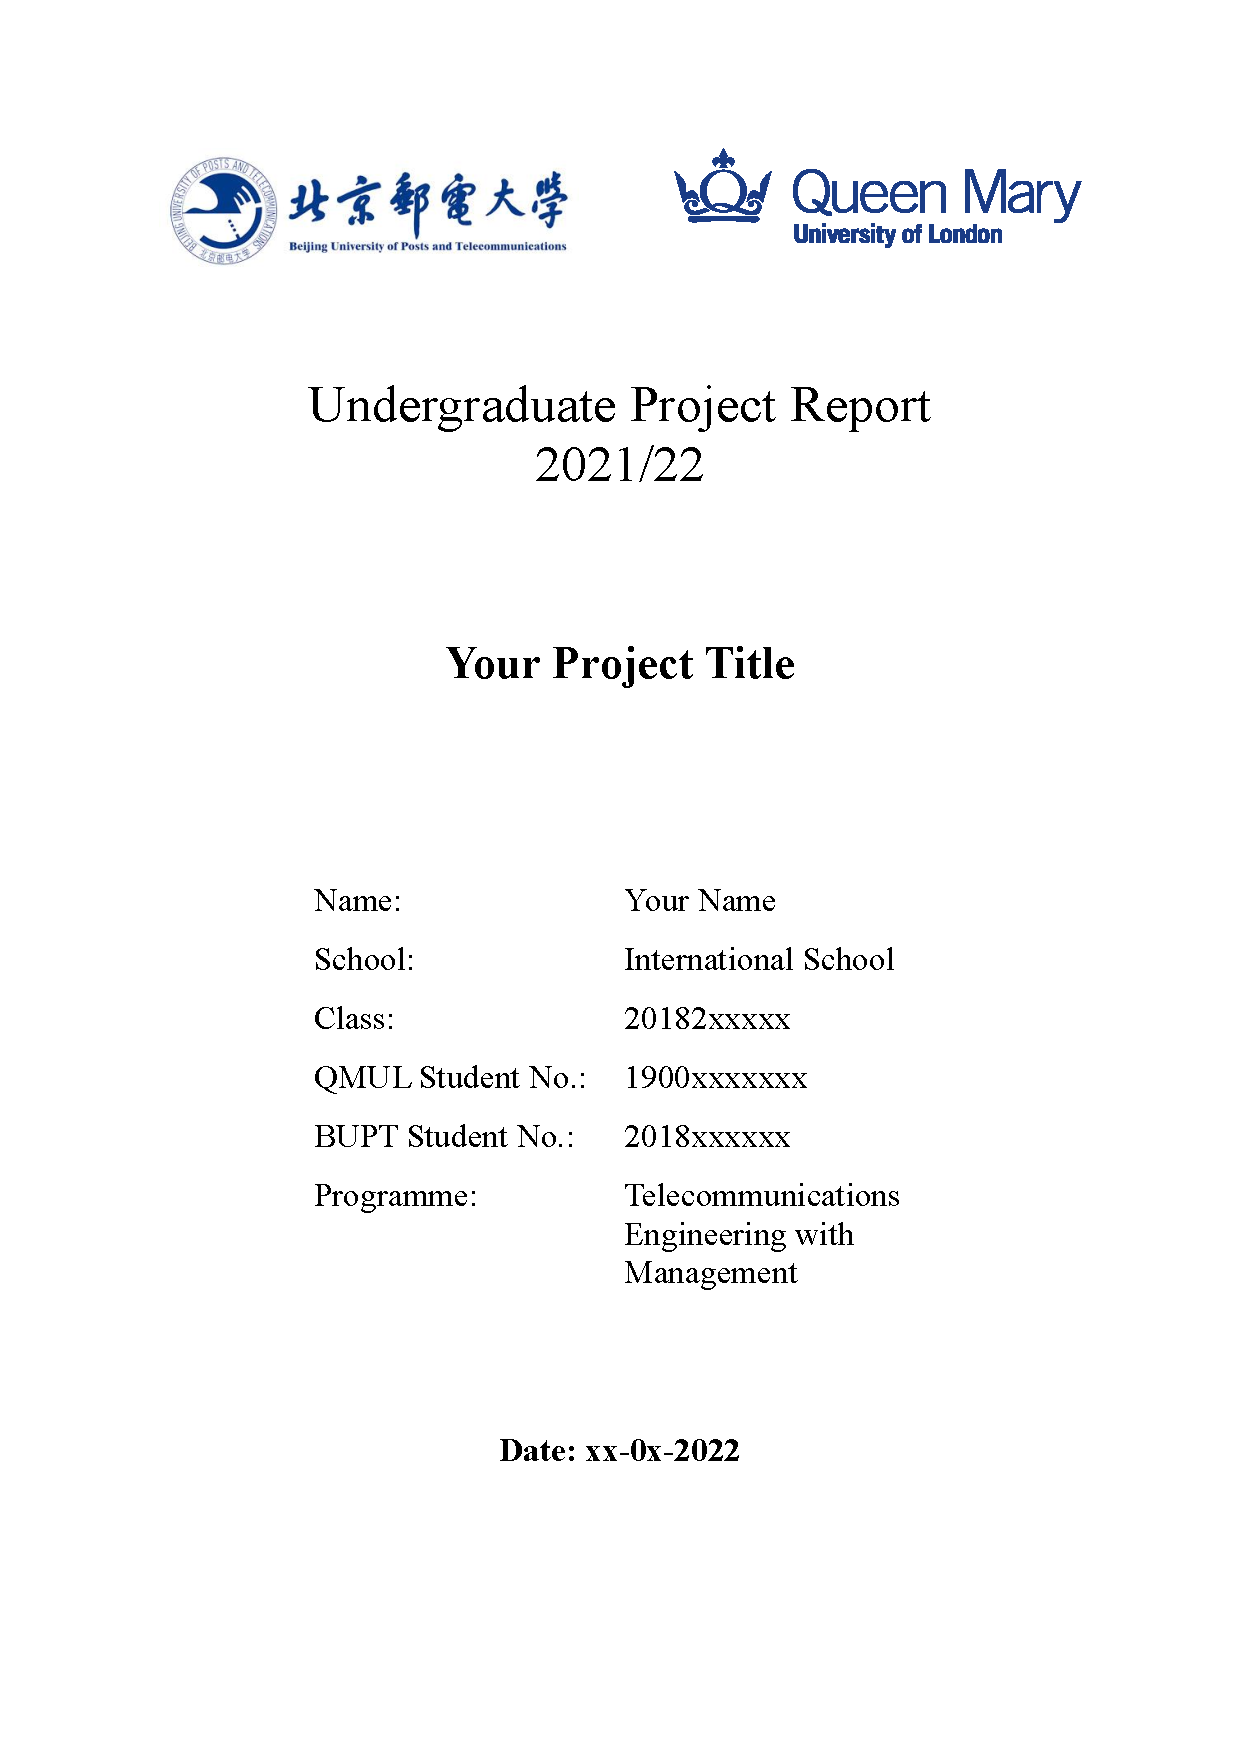
\includepdf[pages=-]{InitialFinalMaterials/TitlePage.pdf}

% \begin{titlepage}

%defines the geometry for the titlepage
\newgeometry{left=40mm, right=40mm, top=40mm, bottom=40mm}  


\begin{center}

% thesis title
%---------------------------------------
\begin{spacing}{2.5}
{\Huge \textsc{\textbf{A socio-economic analysis of the role played by the discovery of ice in the cultural development of Macondo}}}
\end{spacing}

\vspace{1.0 cm}

% QM crest (optional)
%---------------------------------------
% Somewhere in this page you might want QM logo, or University of London logo, or funding body logo
% depending on your exact situation
\begin{center}

\includegraphics[width=0.4\textwidth]{QM_crest}
\end{center}
\vspace{0.9cm}


% author
%---------------------------------------
{\LARGE Clearlove7} % authorS

\vspace{1cm}


% requirements. If unsure about the exact text for your case, 
% contact the Research Degrees Office
{\large \sffamily
Submitted in partial fulfillment of the
requirements \\ of the Degree of Doctor of Philosophy\\
\vspace{0.9 cm}
School of Alchemia\\
\vspace{0.5 cm}
Queen Mary University of London\\
\vspace{0.5cm}
September 4396 % date of submission
}

\end{center}



\end{titlepage}

\restoregeometry  % restores the geometry
\doublespacing		% restores the spacing
%\onehalfspacing
 % titlepage


% Statement of originality
%----------------------------------------------------------
% \chapter*{Statement of originality}
\label{C:Statement}
\addcontentsline{toc}{section}{\nameref{C:Statement}}

I, [insert name as recorded in QM records], confirm that the research included
within this thesis is my own work or that where it has been carried out in
collaboration with, or supported by others, that this is duly acknowledged
below and my contribution indicated. Previously published material is also
acknowledged below.

\bigskip

\noindent
I attest that I have exercised reasonable care to ensure that the work is
original, and does not to the best of my knowledge break any UK law, infringe
any third party’s copyright or other Intellectual Property Right, or contain any
confidential material.

\bigskip

\noindent
I accept that the College has the right to use plagiarism detection software to
check the electronic version of the thesis.

\bigskip

\noindent
I confirm that this thesis has not been previously submitted for the award of a
degree by this or any other university.

\bigskip

\noindent
The copyright of this thesis rests with the author and no quotation from it or
information derived from it may be published without the prior written consent
of the author.

\bigskip

\noindent
Signature: [can be digital signature]

\noindent
Date:

\bigskip

\noindent
Details of collaboration and publications: 

\noindent
[insert details here if applicable]   


% content
\tableofcontents


% Abstract
%----------------------------------------------------------
\chapter*{Abstract}
\label{C:Abstract}
\addcontentsline{toc}{chapter}{\nameref{C:Abstract}}

% no more than 300 words


数学、中英文皆可以混排。You can intersperse math, Chinese and English (Latin script) without adding extra environments.

\newpage

% test

% \vspace{8cm}

\Huge \textbf{摘要}

\vspace{1.5cm}

\normalsize
数学、中英文皆可以混排。You can intersperse math, Chinese and English (Latin script) without adding extra environments.

  



% Epighraph 
%----------------------------------------------------------
% \cleardoublepage
% \thispagestyle{empty}
% \epigraph{O time, thou must untangle this, not I.
% It is too hard a knot for me to untie!}
% {\textit{Twelfth Night}\\
% \textsc{Shakespeare}}

% Acknowledgements and licences
%----------------------------------------------------------
% \chapter*{Acknowledgements}
\label{C:Acknowledgements}
\addcontentsline{toc}{chapter}{\nameref{C:Acknowledgements}}


\begin{otherlanguage}{italian}
\textit{A gloria non si va senza fatica.
}
\end{otherlanguage}





%  Table of contents           
%----------------------------------------------------------
% \tableofcontents
% \listoffigures
% \listoftables



%%------------------------------------------------------------------------------------
%% Beginning of Mainmatter
%%------------------------------------------------------------------------------------




\chapter{Introduction}
\label{ch:intro}

\blindtext


\chapter{Background}
\label{ch:background}
\section{Graph Definition} 
\blindtext


\chapter{Methodology}
\label{ch:method}

\blindtext




\chapter{Experimental Evaluation}
\label{ch:evaluation}

\blindtext


\chapter{Conclusion and Further Work}
\label{ch:con}
\section{Conclusion}
\blindtext






%%------------------------------------------------------------------------------------
%% Appendices 
%%------------------------------------------------------------------------------------
% \appendix % resets chapter numbering, uses letters for appendix chapter numbers

% % Appendix to show those painful calculations and lond tables 
% Here it's just a dummy produced with the blindtext package

% \blindmathfalse
% \blinddocument

\chapter*{Appendix}
\label{ch:appendix}

\addcontentsline{toc}{chapter}{\nameref{ch:appendix}}


%%------------------------------------------------------------------------------------
%% Beginning of Backmatter
%%------------------------------------------------------------------------------------
\backmatter % turns off chapter numbering 


%Bibliografia
%------------------------------------------------------------------
\bibliography{InitialFinalMaterials/Bibliography.bib}{}
% \bibliographystyle{plain}

\chapter*{Acknowledgements}
\label{C:Acknowledgements}
\addcontentsline{toc}{chapter}{\nameref{C:Acknowledgements}}


\begin{otherlanguage}{italian}
\textit{A gloria non si va senza fatica.
}
\end{otherlanguage}




% Appendix to show those painful calculations and lond tables 
% Here it's just a dummy produced with the blindtext package

% \blindmathfalse
% \blinddocument

\chapter*{Appendix}
\label{ch:appendix}

\addcontentsline{toc}{chapter}{\nameref{ch:appendix}}


% \printindex 		% to make the index
\end{document}
